\documentclass{../template/Report}
\settemplatedir{../template/} %设置模板文件夹路径

\exname{声速的测定} %实验名称
\extable{8}
\instructor{刘振武} %指导教师
\class{周三上午} %班级
\name{} %姓名
\stuid{} %学号

\nyear{2025} %年
\nmonth{9} %月
\nday{24} %日
\nweekday{三} %星期几
\daypart{上午}
\redate{} %如有实验补做,补做日期
\resitu{} %情况说明:

\begin{document}
\maketitle

\section{预习报告(10分)}
\subsection{实验综述(5分)}
\subsubsection{实验目的}
\begin{enumerate}
	\item 了解声波的特性,加深对振动合成和波干涉理论的理解
	\item 学会用相位差法和驻波法测定声速在空气中的传播速度
	\item 学习示波器和信号发生器的使用方法
\end{enumerate}
\subsubsection{实验原理}
\begin{enumerate}
	\item 超声波传播速度:声波在理想气体中传播可看作绝热过程,其传播速度$V=\sqrt{\frac{\gamma RT}{M}}$(
	      M为气体摩尔质量,R为普适气体常量,$\gamma$为热容比,T为热力学温度)。
	      在0$\si{\degreeCelsius}$时,$V=\SI{331.45}{\metre\per\second}$。在t$\si{\degreeCelsius}$时,$V_t = 331.45\sqrt{1+\frac{t}{273.15}}\si{\metre\per\second}$。
	      声波在不同介质中传播速度不同。最简单的方法是直接测量声波振动的波长与频率,$V=\lambda f$。
	      $f$由仪器给定,我们仅需使用驻波法(或共振干涉法)或相位比较法测定$\lambda$。
	\item 驻波法测波长:由于入射波和反射波相互叠加,两个波节之间形成共振驻波现象,波幅达到极大值。
	      由于纵波的性质,振动位移处于波节时,声压处于波腹,即接收器端面移动位移为一波节时,接收到的声压最大,经接收器转换的电信号最强。驻波共振条件为:$L_n = n\frac{\lambda}{2}$ (n=1,2,3...)\\
	      将接收信号输入示波器就可看到最大波振幅,
	      接收端每移动距离$\Delta L$使示波器上再次观测到最大波振幅移动距离满足:$\Delta L = L_{n+1} - L_n = n\frac{\lambda}{2}$\\
	      准上式代入$v=\lambda f$,即可得$v$
	\item 相位比较法测波长:沿波传播方向上的任意两点,其振动状态相同,或者说其相位差为$2\pi$的整数倍时,
	      两点间距为$\lambda$的整数倍,利用这一原理可测波长。
	      我们通过移动接收端改变相位差$\Delta\varphi$,使示波器上显示的李萨如图形如下变化,记录下$N$次二、三象限直线或二四象限图形位置读数$L_i$,同样有$\Delta L = L_{n+1} - L_n = \frac{\lambda}{2}$,代入$v=\lambda f$可得$v$
\end{enumerate}
\begin{figure}[H]
	\centering
	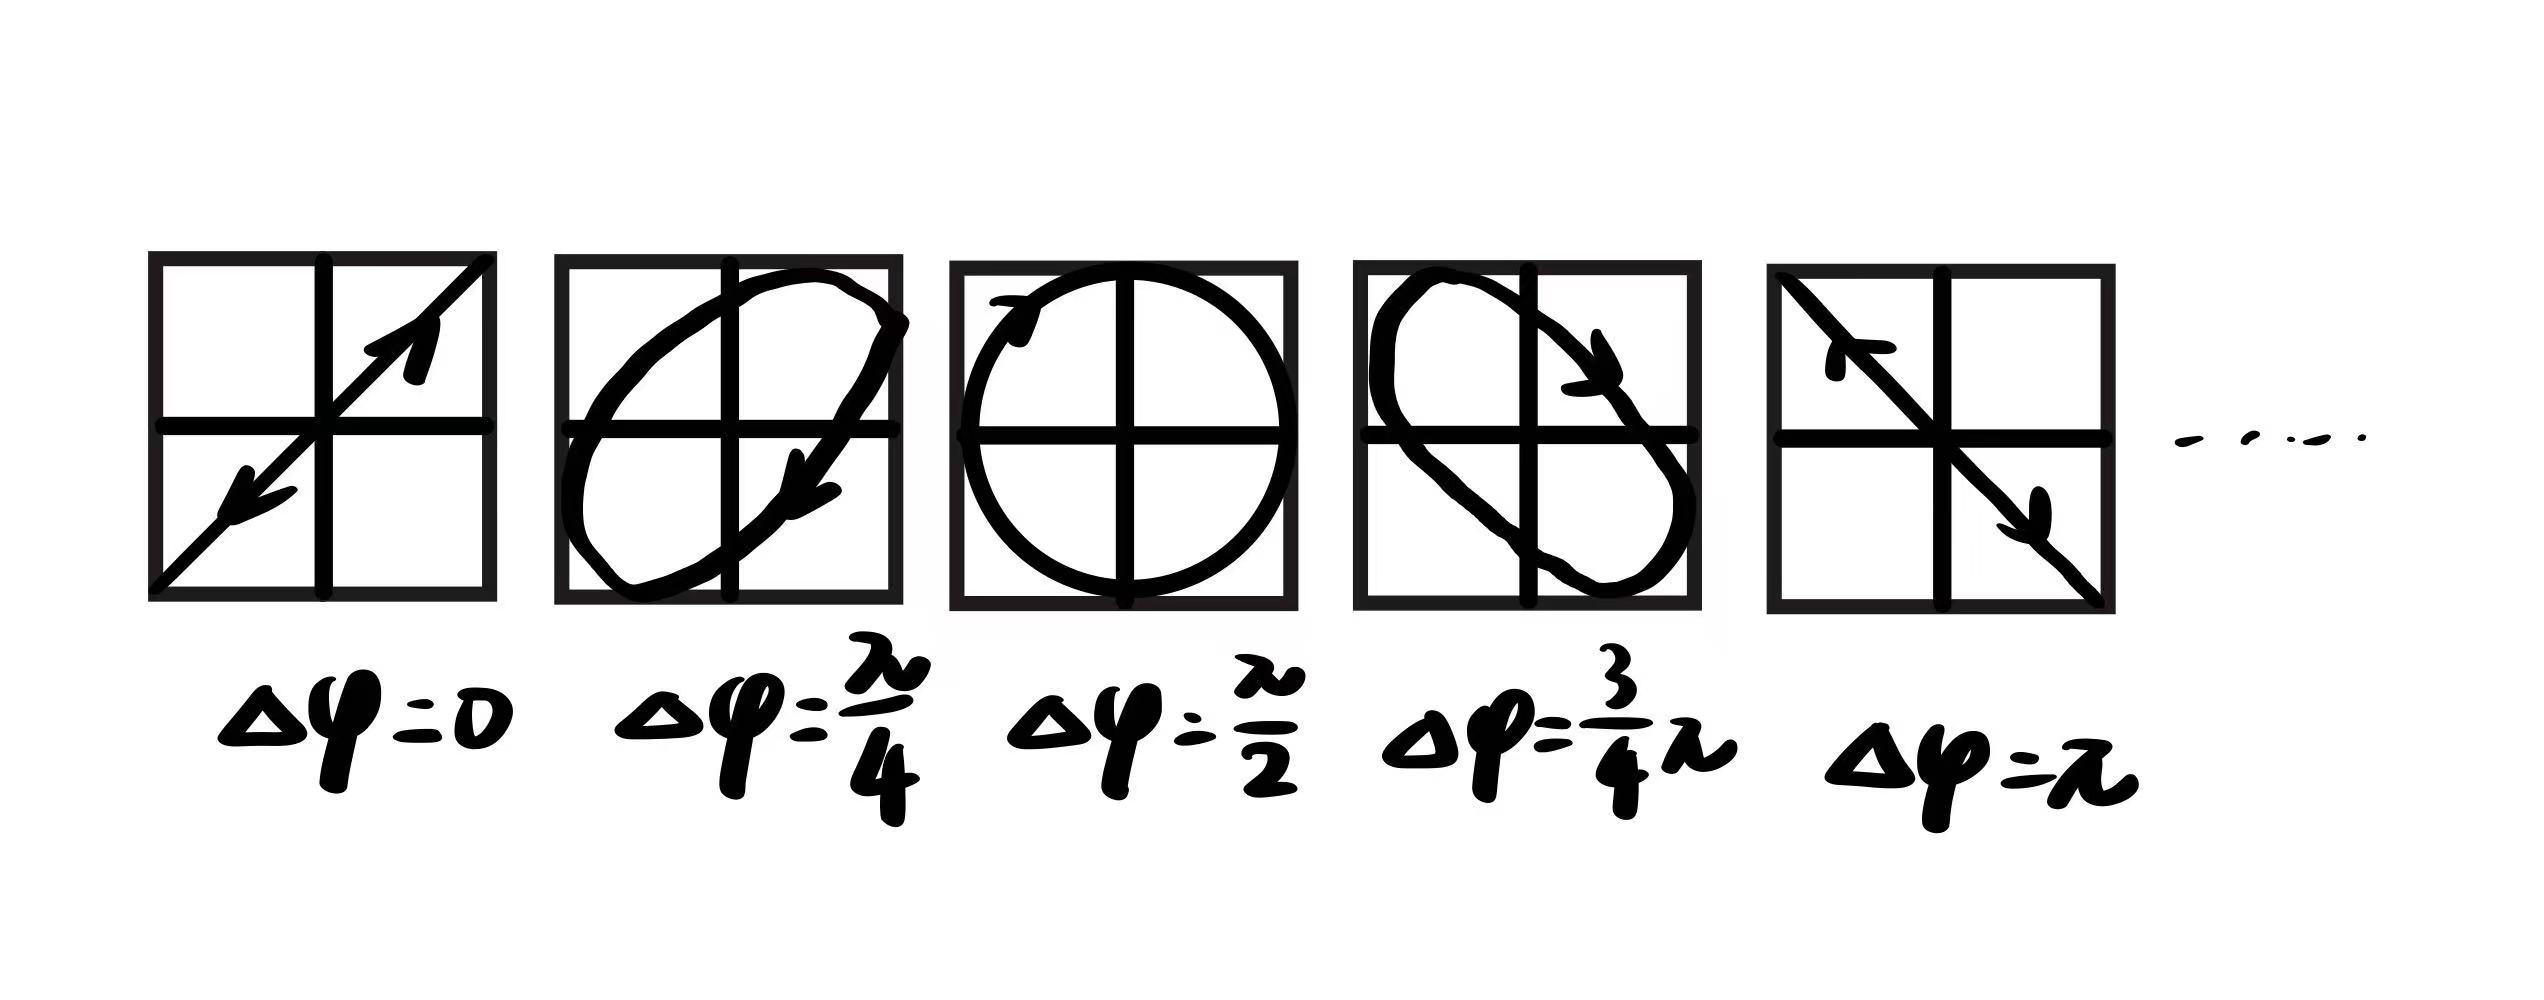
\includegraphics[width=0.8\textwidth]{1.jpg}
	\caption{相位比较法测波长中的李萨如图形}
\end{figure}
\subsection{实验重点(3分)}
% (简述本实验的学习重点,不超过100字。)
\begin{enumerate}
	\item \textbf{系统调节:}实验时只有信号频率与两个具有相同固有频率的换能转换器一致时,

	      \textbf{调节方法:}使移动端与固定端尽量做到并平行,将接收信号输入示波器Y轴,
	      在信号发生器上调节频率旋钮选择谐振频率(约40\si{\kilo\hertz}),然后微调信号发生器的频率旋钮,
	      直到示波器上出现最大振幅,此时显示的频率数值才是实验所需的谐振频率。

	\item \textbf{驻波法测声速:}调节超声换能器至最佳状态后,
	      将移动接收端来回移动,观察干涉现象。缓慢移动接收端,
	      示波器上出现最大振幅波形,从标尺上读得此时的位置读数$L_1$,
	      继续向同一方向移动接收端,逐次记录出现最大振幅的位置$L_i$,连续记录8次,同时记下$f$。
	      若显示频率有细微增减,可读记起始频率$f_1$和结束测量时$f_2$,以$\frac{f_1+f_2}{2}$作为$f$。

	\item \textbf{相位差法测声速:}将发射端的信号输入示波器X轴,
	      选择发射端与接收端两振动信号分别输入示波器X和Y轴的偏转板上,在屏幕上显示了合成后的李萨如图形。
	      移动接收端就可在示波器上看到一、三象限的直线,从标尺上读得此时的位置$L_1$,
	      再像移动接收端,测得在示波器上看到二、四象限的直线,从标尺上读得此时位置读数$L_2$,同时记下此时$f$,连续记录8个数据。
\end{enumerate}
\subsection{实验难点(2分)}
% (简述本实验的实现难点,不超过100字。)
\begin{enumerate}
	\item \textbf{波形变化可能不明显:}尽量使移动端换能器靠近固定端,使波形变化明显。
	\item \textbf{移动接收端方向问题:}移动接收端时必须沿一方向,严禁因相位差超过需读数点而反向移动(如发生则重做实验),否则会产生误差。
	\item \textbf{读数有效位数:}读数时注意有效位数,螺旋测微仪分度值为\SI{0.01}{\mm},故包含估读的读数应到\SI{0.001}{\mm}数量级。
\end{enumerate}

\begin{fullreportonly}
	\section{原始数据(20分)}
	% (将有老师签名的“自备数据记录草稿纸”的扫描或手机拍摄图粘贴在下方,完整保留姓名,学号,教师签字和日期。)
	\begin{figure}[H]
		\centering
		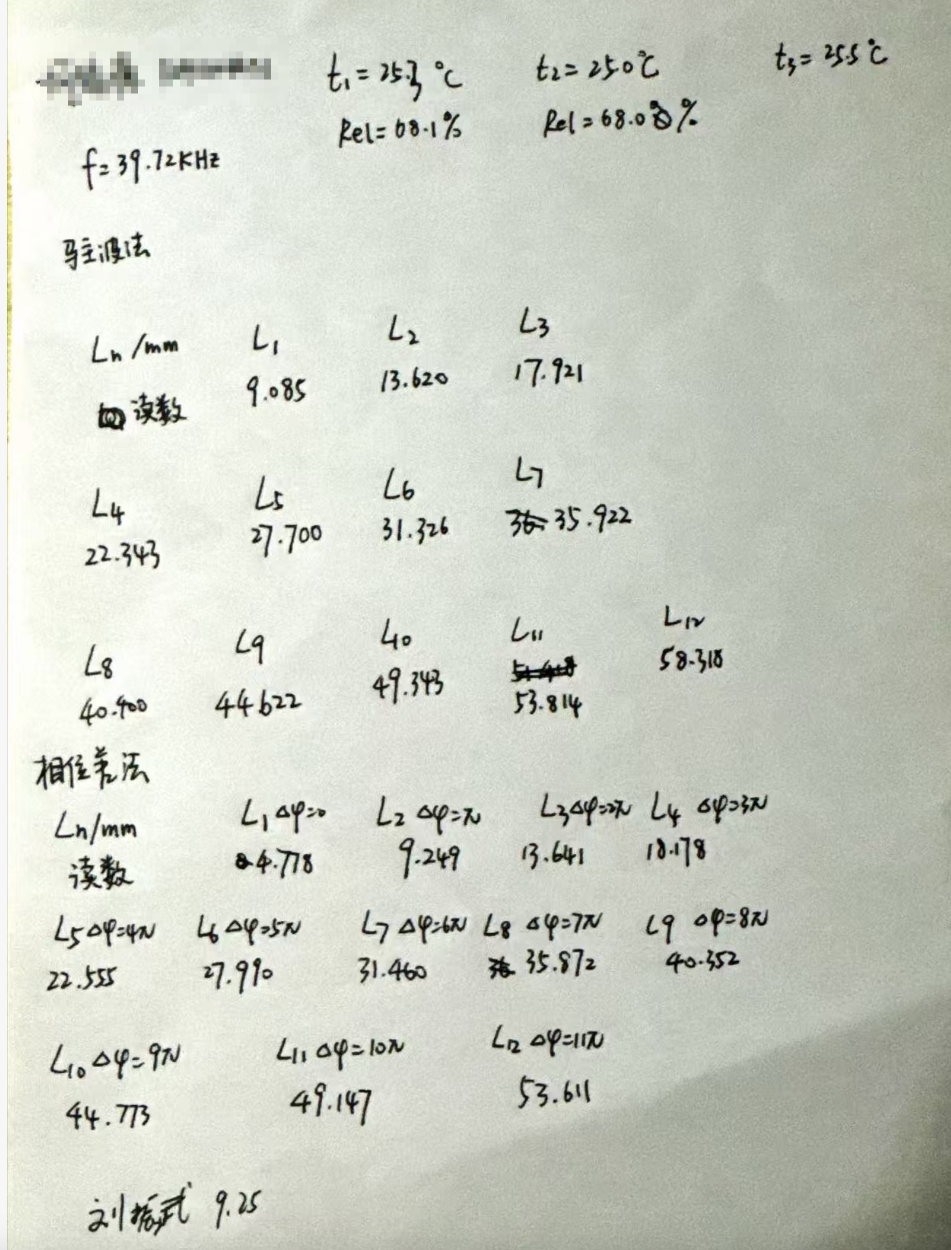
\includegraphics[width=0.8\textwidth]{data.png}
		\caption{实验数据记录}
	\end{figure}
	\section{结果与分析(60分)}
	\subsection{数据处理与结果(30分)}
	% (列出数据表格、选择适合的数据处理方法、写出测量或计算结果。)
	\begin{table}[H]
		\centering
		\caption{实验数据记录表}
		\label{tab:exp_data}
		\begin{tabular}{|c|c|c|C{5em}|C{3em}|c|}
			\hline
			\multicolumn{3}{|c|}{谐振频率 $f = (39.72) \si{\kilo\hertz}$} & \multicolumn{3}{c|}{环境温度 $t_{\text{环}} = (25.3)\si{\degreeCelsius}$}                                                                                                                                  \\
			\hline
			\textbf{组别}                                               & \textbf{驻波法}                                                         & \textbf{接收端位置读数/$\si{\mm}$}           & \textbf{相位差法}             & \multicolumn{2}{|c|}{\textbf{接收端位置读数/$\si{\mm}$}}          \\
			\hline
			1                                                         & $L_1$                                                                & 9.085                                 & $0$                       & $L_1'$                                            & 4.778  \\
			\hline
			2                                                         & $L_2$                                                                & 13.620                                & $\pi$                     & $L_2'$                                            & 9.249  \\
			\hline
			3                                                         & $L_3$                                                                & 17.921                                & $2\pi$                    & $L_3'$                                            & 13.641 \\
			\hline
			4                                                         & $L_4$                                                                & 22.343                                & $3\pi$                    & $L_4'$                                            & 18.178 \\
			\hline
			5                                                         & $L_5$                                                                & 27.700                                & $4\pi$                    & $L_5'$                                            & 22.555 \\
			\hline
			6                                                         & $L_6$                                                                & 31.326                                & $5\pi$                    & $L_6'$                                            &27.990  \\
			\hline
			7                                                         & $L_7$                                                                & 35.922                                & $6\pi$                    & $L_7'$                                            & 31.460 \\
			\hline
			8                                                         & $L_8$                                                                & 40.400                                & $7\pi$                    & $L_8'$                                            & 35.872 \\
			\hline
			9                                                         & $L_9$                                                                & 44.622                                & $8\pi$                    & $L_9'$                                            & 40.352 \\
			\hline
			10                                                        & $L_{10}$                                                               & 49.343                                & $9\pi$                    & $L_{10}'$                                           & 44.773 \\
			\hline
			11                                                        & $L_{11}$                                                               & 53.814                                & $10\pi$                    & $L_{11}'$                                           & 49.147 \\
			\hline
			12                                                        & $L_{12}$                                                               & 58.318                                & $11\pi$                    & $L_{12}'$                                           & 53.611 \\
			\hline
			\multicolumn{2}{|c|}{$\bar{\lambda}$}                     & \multicolumn{1}{|c|}{$\SI{8.912}{\mm}$}                                            & \multicolumn{1}{|c|}{$\bar{\lambda}$} & \multicolumn{2}{|c|}{$\SI{8.823}{\mm}$}                                                              \\
			\hline
			\multicolumn{2}{|c|}{$v$}                     & \multicolumn{1}{|c|}{\SI{354.0}{\meter\per\second}}                                            & \multicolumn{1}{|c|}{$v$} & \multicolumn{2}{|c|}{$\SI{350.5}{\meter\per\second}$}                                                              \\
			\hline
		\end{tabular}
	\end{table}
	\subsubsection{声速的理论值计算}
	\begin{align*}
		\bar{t}        & = \cfrac{25.3 + 25.0 + 25.5}{3}                    = 25.3\si{\degreeCelsius}     \\
		v_{ \text{声} } & = 331.45 \cdot \sqrt{1 + \cfrac{\bar{t}}{273.15}}  = \SI{346}{\meter\per\second}
	\end{align*}
	\subsubsection{用两种方法测声速计算}
	\paragraph{驻波法}
	由\cref{tab:exp_data}可得
	\begin{align*}
		\frac{\lambda}{2}&=\frac{(L_{12}+L_{11}+L_{10}+L_9+L_8+L_7)-(L_6+L_5+L_4+L_3+L_2+L_1)}{6\times6}=4.456 \si{mm} \\
		\bar{\lambda} &= 8.912 \si{mm} \\
		v_1 &= \lambda \cdot f = 8.912 \times 10^{-3} \times 39.72 \times 10^{3} = 354.0 \si{\meter\per\second}\\
		\mathrm{E}_1 &= \cfrac{\left|v_1 - v_{\text{声}}\right|}{v_{\text{声}}} = 2.31\%
	\end{align*}
	\paragraph{相位差法}
	由\cref{tab:exp_data}可得
	\begin{align*}
		\frac{\lambda}{2}&=\frac{(L_{12}+L_{11}+L_{10}+L_9+L_8+L_7)-(L_6+L_5+L_4+L_3+L_2+L_1)}{6\times6}=4.411 \si{mm} \\
		\bar{\lambda} &= 8.823 \si{mm} \\
		v_1 &= \lambda \cdot f = 8.823 \times 10^{-3} \times 39.72 \times 10^{3} = 350.5 \si{\meter\per\second}\\
		\mathrm{E}_1 &= \cfrac{\left|v_1 - v_{\text{声}}\right|}{v_{\text{声}}} = 1.30\%
	\end{align*}
	\subsection{误差分析(20分)}
	\begin{enumerate}
    \item 驻波法在确定振幅最大值时存在较大的主观性。由于振幅在峰值附近变化不显著,实验者可能将最大值所在区间内的任意点作为读数,从而引入误差。为提高测量精度,可以记录峰值开始变大时的$L_1$和峰值开始变小时的$L_2$,取其平均值作为读数。
    \item 相位差法依赖于对两条波形重合的目视判断,两条线是否重合的判断同样存在主观性,是系统误差的一个来源。
    \item 实际实验中,输出频率会有上下波动,且$X, Y$轴示波波动时也会导致图形变化,使判断产生影响。
    \item 在使用螺旋测微器时,读数时视线不一定正对刻度线,使读数时有一定误差。
	\end{enumerate}

	\subsection{实验探讨(10分)}
	% (对实验内容、现象和过程的小结,不超过100字。)
	通过本次实验,我了解了声波的基本特性,掌握了信号发生器的使用,示波器的使用以及驻波法和相位差法测定声速的原理和方法。驻波法中,通过寻找振幅最大的值找到半波长,进而计算出声速;相位差法则是通过示波器上显示的李萨如图形的变化来测定声速。
	在实验过程中,老师提到了测量的过程中不能回调,防止齿轮空程差带来的误差,这让我意识到在实验中需要注意仪器的使用方法和可能存在的误差来源。
	\section{思考题(10分)}
	% (解答教材或讲义或老师布置的思考题,请先写题干,再作答。)
	\subsection{同频率两相互垂直的振动合成中,当相位差为$2\pi$的整数倍时,李萨如图形为一、三象限的直线,当相位差为$\pi$的奇数倍时是二、四象限的直线。试证明之。}
	证明如下:
	\begin{align*}
		&\text{当两者相位差为}2k\pi\text{时},x = A\sin(\omega t), y = A\sin(\omega t + 2k\pi) = x \\
		&\text{即:}y = x, \text{图像过一三象限;}\\
		&\text{当两者相位差为}(2k + 1)\pi\text{时},x = A\sin(\omega t), y = A\sin(\omega t + 2k\pi + \pi) = -x \\
		&\text{即:}y = -x, \text{图像过二四象限;}\\
	\end{align*}
	\subsection{实验前为什么要调整测试系统的谐振频率?}
	在谐振时,信号的振幅更大,波形变化更明显,更容易观察到驻波和相位差的变化,从而使得实验误差更小。
	\subsection{如果超声波发生器$\bar{f}$ = \SI{40}{\kilo\hertz},不确定度$u_f = \SI{10}{\hertz}$, 测$\lambda$时引起的波长的不确定度为$\u_{\lambda} = \SI{0.030}{\mm}$, $\bar{\lambda} = \SI{8.560}{\mm}$, 则实验中所测得的声速相对不确定度$\frac{u_v}{v}$可达多少?}
	\begin{equation*}
		\cfrac{u_v}{v}  = \sqrt{\left(\cfrac{u_f}{\bar{f}}\right)^2 + \left(\cfrac{u_{\lambda}}{\bar{\lambda}}\right)^2} = 3.5 \times 10^{-3}
	\end{equation*}

\end{fullreportonly}

\insertnotes
\end{document}
